\documentclass[tikz,convert={outfile=\jobname.svg}]{standalone}
\usetikzlibrary{automata, arrows.meta, positioning}
\begin{document} 
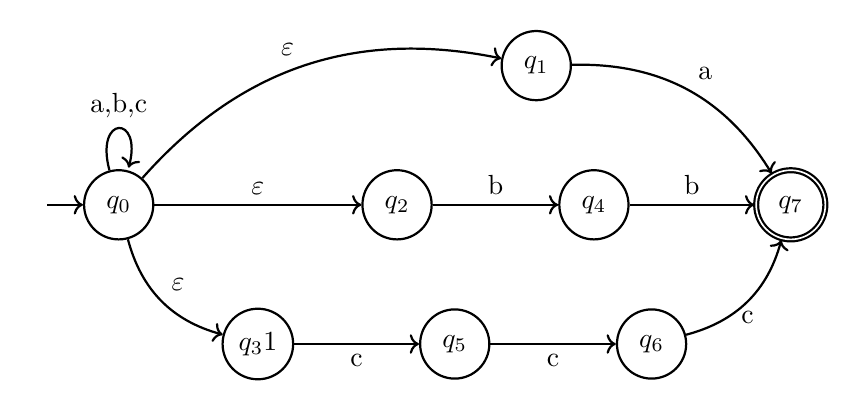
\begin{tikzpicture}[
    thick,
    node distance={25mm},
    auto
]

\node[state, initial, initial text = {}] (q0) {$q_0$}; 
\node[state] (q3) [below right of=q0] {$q_31$}; 
\node[state] (q2) [above right of=q3] {$q_2$}; 
\node[state] (q1) [above right of=q2] {$q_1$}; 
\node[state] (q4) [right of=q2] {$q_4$}; 
\node[state] (q5) [right of=q3] {$q_5$}; 
\node[state] (q6) [right of=q5] {$q_6$}; 
\node[state, accepting] (q7) [above right of=q6] {$q_7$};

\path[->]
    (q0) edge [loop above] node [above] {a,b,c} (q0)
    (q0) edge [bend left] node [] {$\varepsilon$} (q1)
    (q0) edge [] node [] {$\varepsilon$} (q2)
    (q0) edge [bend right] node [] {$\varepsilon$} (q3)
    (q1) edge [bend left] node [] {a} (q7)
    (q2) edge [] node [] {b} (q4)
    (q4) edge [] node [] {b} (q7)
    (q3) edge [] node [below] {c} (q5)
    (q5) edge [] node [below] {c} (q6)
    (q6) edge [bend right] node [below] {c} (q7)
    ;

\end{tikzpicture} 
\end{document}
